\documentclass[]{article}
\usepackage[round]{natbib}

\usepackage{fullpage}
\usepackage[parfill]{parskip}
\usepackage{listings}
\usepackage{url}
\usepackage{authblk}
\usepackage{graphicx}
\usepackage{color}
\usepackage{booktabs}

\lstset{language=Python}

% local definitions
\newcommand{\comment}[1]{{\textcolor{red}{Comment: #1}}}
\newcommand{\aprcomment}[1]{{\textcolor{blue}{APR: #1}}}

\usepackage{xspace}
\newcommand{\GEVA}{\texttt{GEVA}\xspace}
\newcommand{\tsdate}{\texttt{tsdate}\xspace}
\newcommand{\relate}{\texttt{Relate}\xspace}

% cross-reference with supplement
\usepackage{xr}
\externaldocument{supplement}

\begin{document}

\title{On the fraught inference of historical generation times}
\author[1,*]{Aaron P. Ragsdale}
\author[2]{Kevin Thornton}
\affil[1]{University of Wisconsin--Madison, Wisconsin, USA}
\affil[2]{University of California, Irvine, California, USA}
\affil[*]{email@address.edu}
\maketitle

\begin{abstract}

    \noindent \citet{wang2023human} recently proposed an approach to infer the
    history of human generation times from changes in mutation profiles over
    time. With the observation that the relative proportions of different
    mutation types depend on the ages of parents, stratifying variants by the
    age of mutation allows for the inference of average paternal and maternal
    generation times at past times. Applying this approach to published allele
    age estimates, \citeauthor{wang2023human} inferred long-lasting sex
    differences in average generation times and surprisingly found that
    ancestral generation times of West African populations remained
    substantially higher than those of Eurasian populations extending tens of
    thousands of generations into the past. Here we show that the results and
    interpretations in \citet{wang2023human} are driven by noise and biases in
    input data, questionable modeling and statistical choices, and a failure to
    validate their inferences using independent approaches for estimating
    allele ages. With the recent development of methods to reconstruct
    genome-wide gene genealogies, coalescence times, and allele ages, we
    caution that ...

    \aprcomment{this seems kind of aggressive\ldots just writing down some thoughts}

\end{abstract}

Recent years have seen the rapid development of methods for reconstructing
genealogical structures of large cohorts
\citep{speidel2019method,wohns2022unified,hubisz2020mapping}, which are
comprised of a series of gene genealogies (or trees) along the genome.
Reconstructed genealogies (or informative summaries of them
\citep{albers2020dating}) have the potential to transform evolutionary and
population genetic inference, as biological and evolutionary processes impact
the shape and correlation of gene trees and the distribution of variation that
arises in the lineages they represent. Relevant to this study, the age of a
variant can be estimated by mapping its mutation to the portion of the gene
tree in which it is inferred to have occurred.

At the same time, the last few years have seen large sequencing projects that
provide ever-increasing resolution of genome biology, including direct
measurements of mutation rates and profiles
\citep{jonsson2017parental,halldorsson2019characterizing}. Through
high-coverage sequencing of multiple generations of families, \emph{de novo}
mutations can be determined as maternally or paternally inherited, and with a
large enough sample size both the number of mutations and proportions of
mutation types (e.g., A$\rightarrow$C, A$\rightarrow$G, etc.) can be correlated
with parental age and sex \citep{jonsson2017parental}. \citet{wang2023human}
combined these two sets of inferences, the estimated ages of mutations and the
parental age- and sex-dependence of the mutation spectrum, to infer the history
of average maternal and paternal generation intervals for human populations of
diverse ancestries. In order to avoid overfitting, this approach requires
making a number of assumptions about the constancy of the mutational process
\cite{harris,dewitt} \aprcomment{and others to point out? For now, let's accept
these as stated\ldots}

\subsection*{Long-lasting differences in human generation intervals}

In applying this inference approach to multiple populations of different
continental ancestries, \citet{wang2023human} estimated that the ancestors of
European, East Asian, and South Asian populations included in the
\citet{1000genomes2015} dataset (1KGP) have a history of significantly reduced
average generation times compared to West African populations. These
differences extend to over 10,000 generations, the time period highlighted in
this study. In discussing this result the authors state, ``the difference
among populations beyond 2000 generations ago reflects population structure in
humans before their dispersal out of Africa, a structure that is not fully
captured by the 1000 Genomes AFR sample. This implies that the simple labels
of `African' and `non-African' for these populations conceal differences in
generation times that existed on our ancestral continent.'' Indeed, a number of
recent genetic studies suggest that human population structure within Africa
extending hundreds of thousands of years into the past has in part shaped
modern-day genetic variation
\citep{plagnol2006possible,hammer2011genetic,hsieh2016model,hey2018phylogeny,
ragsdale2019models,durvasula2020recovering,lorente2019whole}.

However, in extending their analysis farther into the past,
\citeauthor{wang2023human} find that ancestral generation intervals do not
converge until many 10s of thousands of generations age. With an average
generation time of 25--30 years, this corresponds to well over one million
years ago. This observation would require some portion of the ancestries of
Eurasian and West African populations to have remained isolated for many
hundreds of thousands of years, for those structured ancestral populations to
have had large differences in average generation times over the course of this
history, and for those groups to have contributed substantively to different
contemporary human populations. While such a scenario of very long-lasting
isolation among ancestral popualtions is not impossible, it is not supported by
genetic \citep{ragsdale2022weakly,others} or archaeological
\citep{scerri2018did,others} evidence, which rather suggest at least periodic
connectivity of ancestral human populations within Africa.

Rather than long-lasting isolation between a large portion of ancestry of West
African and Eurasian populations (that represented large differences in
generation intervals), Eurasian--West African divergence has been estimated at
only $\approx 75$ka (thousand years ago)
\citep[e.g.,][]{pagani2015tracing,other}. Even studies that have inferred
deeper divergences of human populations within African would place the
Eurasian--West African divergence at around 100--150ka
\citep{schlebusch2017southern}. 

\aprcomment{
    If these estimated divergences represents the majority of ancestry of the
    two populations, can we do a back of the envelope calculation to see what
    difference in generation time would be needed between the hypothesized
    minority of deeply structured ancestry contributing to these pops in order
    to explain the estimated average differences in generation times? I bet it
    would be huge.
}

Given the implausibility of the stated result, it is natural to ask what may be
causing such mis-inferences. Below we show that multiple sources of uncertainty,
namely noise and bias in allele age inference and incosistencies in trio-base
estimates of mutation profiles, confound inferences of generation times from
time series of mutation spectra.

\subsection*{Inconsistencies in inferred mutation spectra over time}

Central to the inference of generation intervals from time-stratified mutation
spectra is the dating of variant ages. \citet{wang2023human} used published
allele ages from \citet{albers2020dating} (using the software \GEVA).
\GEVA estimates allele ages by considering the number of additional
mutations that have accumulated on the ancestral haplotype carrying the focal
variant, as well as the effect of recombination in reducing the size of that
ancestral haplotype. Singletons are excluded from analysis by \GEVA and
are not assigned an age. Partitioning variants by their estimated ages shows
that the mutation spectrum (i.e., the distribution of six mutation types) has
changed over time, assuming that the observed spectrum of segregating variation
is not biased with respect to the spectrum of \emph{de novo} mutations occuring
during that time (Figure~\ref{fig:xyz} and see Figure 1C in
\citeauthor{wang2023human}). \aprcomment{Would require a selection (or
genotyping error) argument.}

Focusing on the \GEVA data,
\begin{itemize}
    \item Beyond 10,000 generations, \GEVA-ages spectra fluctuate by a
        very large amount (although \citet{wang2023human} ``note that age
        estimates of mutations in the very distant past have decreased
        accuracy.'')
    \item The fit is poor between data and model predictions, with model
        spectra trending in opposite directions from the data for some
        mutation classes \citep{gao2022limited}
\end{itemize}

Given the poor fit of the model to the data and the known uncertainty in age
estimation for older variants \citep{albers2020dating}, we attempted to
reproduce the inferred generation interval histories using allele age estimates
from independent methods, names \relate \citep{speidel2019method} and \tsdate
\citep{wohns2022unified}, two state-of-the-art genealogical reconstruction
methods.
\begin{itemize}
    \item Allele age estimates between the three methods are only moderately
        correlated (as shown in Figure S20 in the Supplement of
        \citet{wohns2022unified}).
    \item TODO: estimate this correlation from our parsed data
    \item Despite this low correlation, we would hope that differences are
        unbiased with respect to the age-stratified mutation spectra. However,
        allele ages provided by each method result in distinct and
        unalike mutation spectrum histories (Figures
        \ref{fig:geva-spectra}--\ref{fig:relate-spectra}), with mutation
        spectrum changes often trending in opposite directions over the same
        epochs.
    \item In turn, these divergent histories provide estimates of
        generation time profiles that qualitatively differ.
\end{itemize}

Conclusions from this section:
\begin{itemize}
    \item Mutation spectrum histories stratified by estimated allele ages are
        unreliable, as methods disagree even for fairly young mutations,
        and it's not clear whether \emph{any} of the methods get
        it right (relevant to \citet{gao2022limited}).
    \item It is not obvious where the discrepancies are coming from (need
        to look into \citet{brandt2022evaluation})
\end{itemize}

\subsection*{Mutation spectra differ between \emph{de novo} mutations and young
alleles}

The large disagreements in mutation spectrum histories between multiple variant
age-estimation methods should cause skepticism of down-stream inferences that
rely on them. But if we were to accept one of the mutation spectrum histories
as accurate, there is a further cause for concern in comparing age-stratified
mutation spectra to those estimated from pedigree studies
\citep{jonsson2017parental,halldorsson2019characterizing}. As
\citet{wang2023human} acknowledge, the spectrum of \emph{de novo} mutations
identified in Icelandic trios \citep{jonsson2017parental} differs considerably
from the spectrum of young segregating variation (e.g., variants estimated to
be less than 100 generations old, Table~\ref{tab:recent-spectra}).
\aprcomment{what do \citet{gao2022limited} say is the reason they abandon
them?}

For some mutation classes, the relative proportion of \emph{de novo} mutations
in the trio-based study differs from the young-variant spectrum by up to
$0.05$. Instead, \GEVA, \tsdate, and \relate, while they differ for mutations
that are estimated to be older, very closely agree for mutations inferred to be
less than 100 generations old. In discussing this discrepancy,
\citet{wang2023human} state, ``We found that the mutation spectrum from the
large pedigree study consistently differed from the variant spectrum inferred
from the 1000 Genomes Project data, possibly because we removed singletons from
the polymorphism dataset to reduce errors.'' Rather, \GEVA does not provide
estimates of allele ages for singletons, so this suggested source of
discrepancy cannot be checked with their published allele ages. Both \tsdate
and \relate do report allele ages for singletons, and their inclusion does not
strongly affect the mutation spectrum in the most recent time period
(Table~\ref{tab:recent-spectra}), though it does impact the mutation spectra in
older time periods (Figures~\ref{fig:relate-spectra-singletons},
\ref{fig:tsdate-spectra-singletons}). \aprcomment{also should double check that
the young-variant spectrum is close between a bunch of different populations.}
\aprcomment{Comment on coverage: \GEVA and \relate use the low-coverage 1KGP
data, while \tsdate uses the more recent high-coverage 1KGP data.}

What could be driving the large disagreement between the spectrum of \emph{de
novo} mutations from pedigree-based approaches and that of young variants in
the 1KGP dataset?
\begin{itemize}
    \item True differences in mutation spectrum between the Iceland population
        and 1KGP populations \aprcomment{not likely -- populations of different
        ancestries in 1KGP are consistent, and the EUR populations differ from
        Iceland}
    \item Extremely recent large-scale changes in the \emph{de novo} mutation
        spectrum \aprcomment{also not likely to occur at this scale, but if it
        were true, we should not be using the Iceland trio data to calibrate
        population genetics models at all}
    \item Differences in selective pressures between mutations of different
        classes \aprcomment{selection would need to be very different, and
        affect many variants genome-wide. How strong would selection need
        to be to decrease certain mutation classes by a given amount? We could
        use \emph{moments} for this\ldots}
    \item Genotyping error or bioinformatics choices \aprcomment{the agreement
        between high and low coverage data suggests that genotyping error does
        not have a strong effect in the 1KGP data.} \aprcomment{instead, filtering
        and bioinformatics choices in the pedigree approach are the likely
    culprit.} \citep{bergeron2022mutationathon}

\end{itemize}

Finally, a paragraph on model choices:
\begin{itemize}
    \item I also don't think the approach they took is satisfying:
        \begin{quote}
            Therefore, to obtain absolute generation times for historical
            periods, we centered the observed spectra on the most recent bin,
            subtracting its difference with the average mutation spectrum
            estimated in (14) from each historical spectrum.  This has the
            effect of assuming that parental ages in the pedigreed mutation
            dataset reflect generation times in the most recent historical bin.
        \end{quote}
        And I don't know what biases this introduces. It does have the effect
        of forcing recent bins to have roughly the same inferred average
        generation times for mothers and fathers as the iceland trio data
        ($28.2$ and $32$, resp.). It's therefore not a \emph{result} that
        recent time periods match other estimates. It's a built-in assumption
        of their model
\end{itemize}

\subsection*{Conclusions}

\begin{enumerate}
    \item Allele age estimates are noisy, and probably shouldn't be used
        for such detailed inferences. You'll end up fitting the noise and
        bias of each method.
    \item DNM estimates from trios have their own sets of problems. Do we
        know where the discrepancy between trio-estimated DNM spectrum and
        observations from pop-gen data come from? Probably needs to be
        sorted out.
    \item Finally, \citet{wang2023human} gives us an excellent exmaple of the
        need for validation in population genetics studies, especially when
        inferences are built upon previous inferences that are known to be
        noisy and that need additional validations in their own right.
\end{enumerate}

\break

\subsection*{Figures}

Many of these to the supplement.

\begin{figure}[ht!]
    \centering
    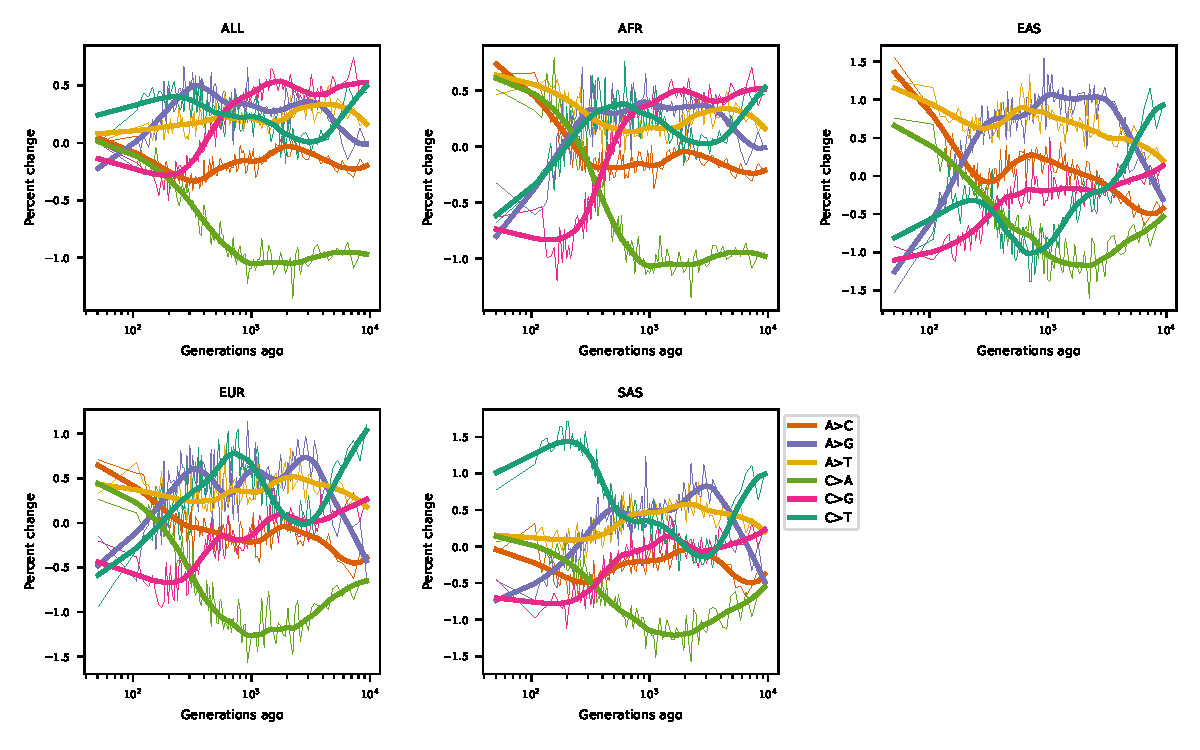
\includegraphics[width=0.8\textwidth]{../plots/spectrum_history.geva.max_age.10000.pdf}
    \caption{
        \textbf{\GEVA-inferred mutation spectrum history.}
    }
    \label{fig:geva-spectra}
\end{figure}


\begin{figure}[ht!]
    \centering
    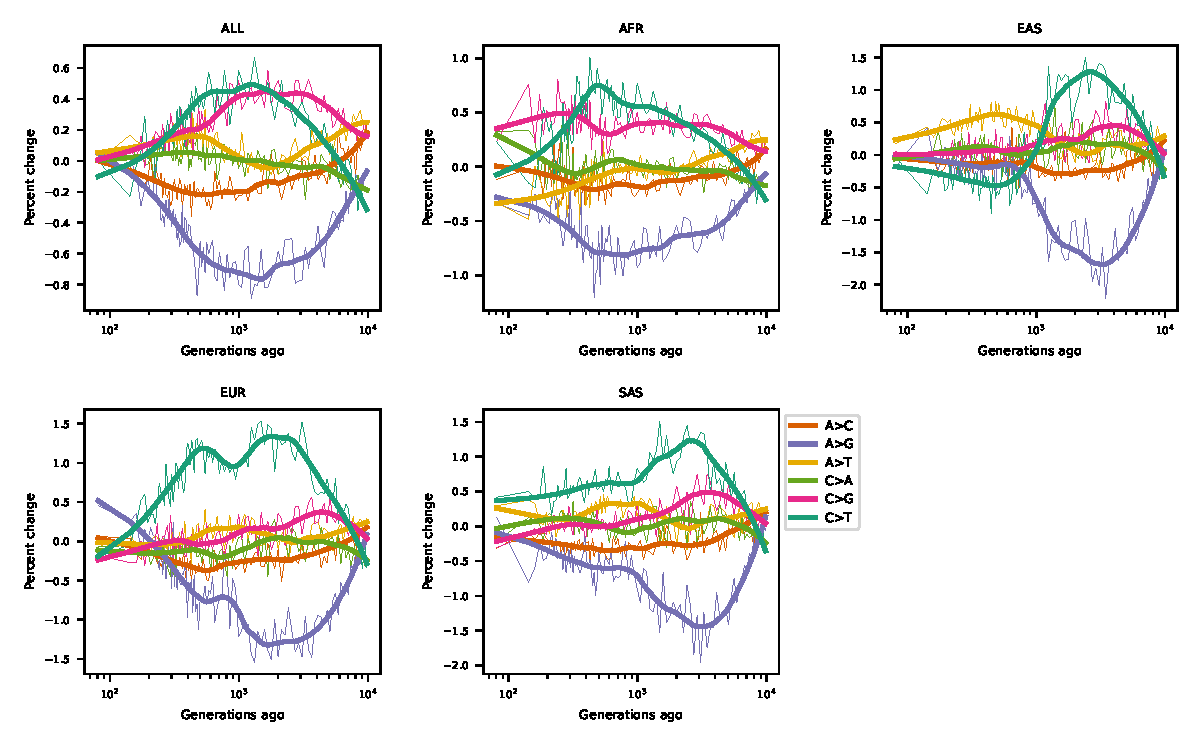
\includegraphics[width=0.8\textwidth]{../plots/spectrum_history.relate.max_age.10000.pdf}
    \caption{
        \textbf{\relate-inferred mutation spectrum history.}
    }
    \label{fig:relate-spectra}
\end{figure}


\begin{figure}[ht!]
    \centering
    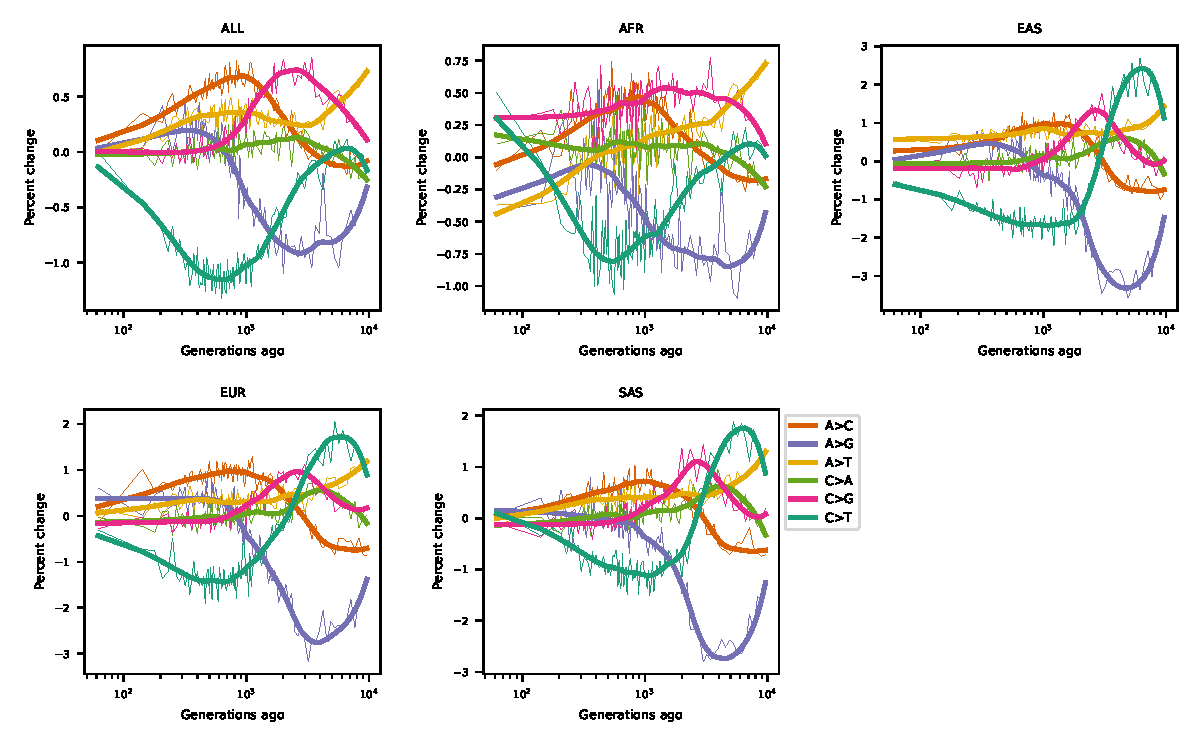
\includegraphics[width=0.8\textwidth]{../plots/spectrum_history.tsdate.max_age.10000.pdf}
    \caption{
        \textbf{\tsdate-inferred mutation spectrum history.}
    }
    \label{fig:tsdate-spectra}
\end{figure}


\begin{figure}[ht!]
    \centering
    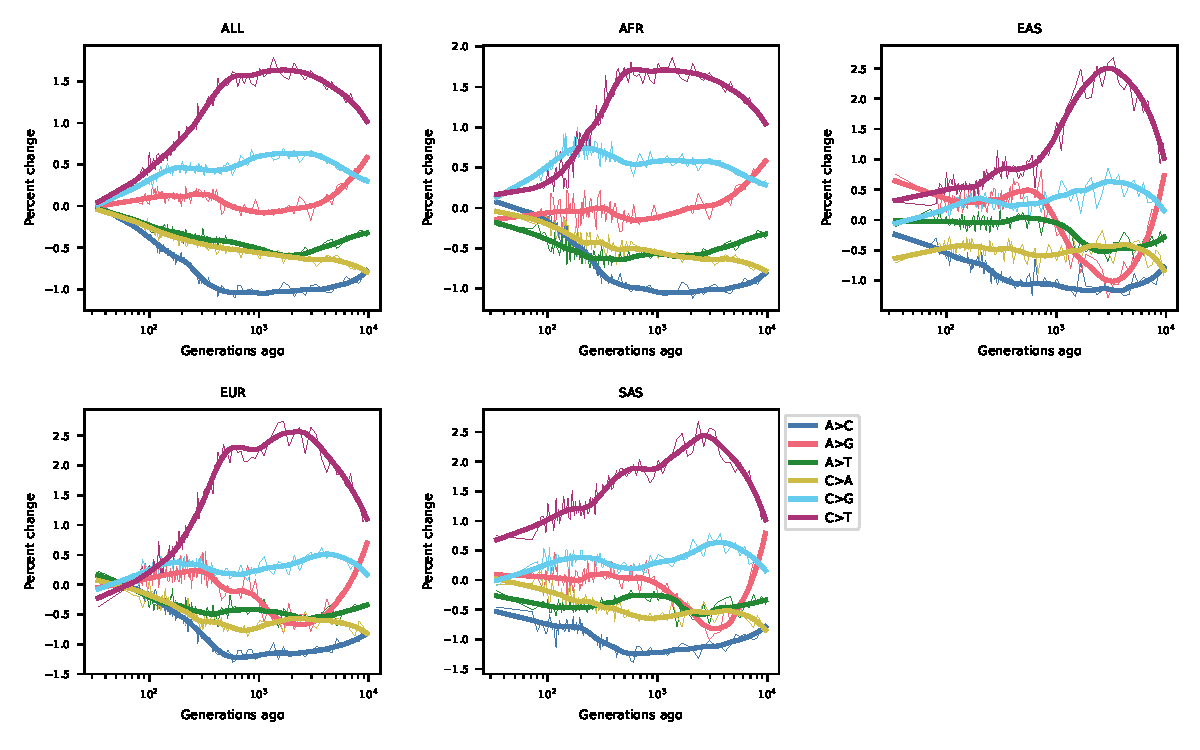
\includegraphics[width=0.8\textwidth]{../plots/spectrum_history.relate.max_age.10000.singletons.pdf}
    \caption{
        \textbf{\relate-inferred mutation spectrum history, including singletons.}
    }
    \label{fig:relate-spectra-singletons}
\end{figure}


\begin{figure}[ht!]
    \centering
    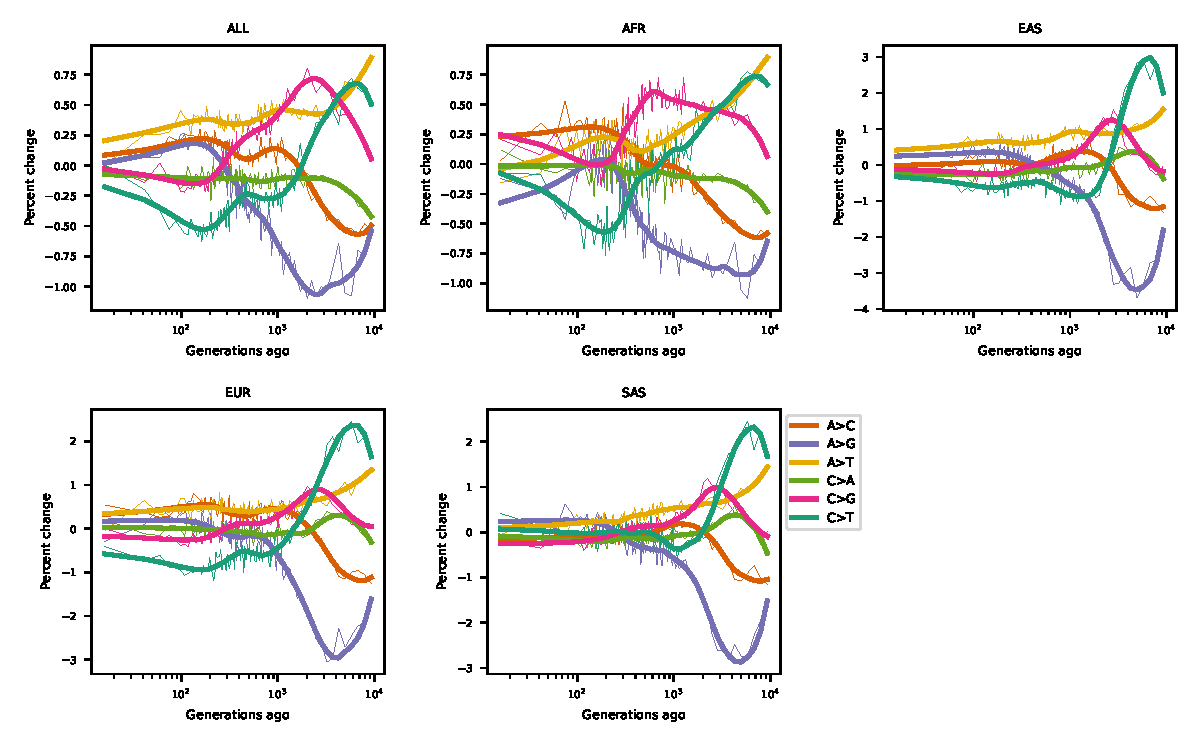
\includegraphics[width=0.8\textwidth]{../plots/spectrum_history.tsdate.max_age.10000.singletons.pdf}
    \caption{
        \textbf{\tsdate-inferred mutation spectrum history, including singletons.}
    }
    \label{fig:tsdate-spectra-singletons}
\end{figure}


\begin{figure}[ht!]
    \centering
    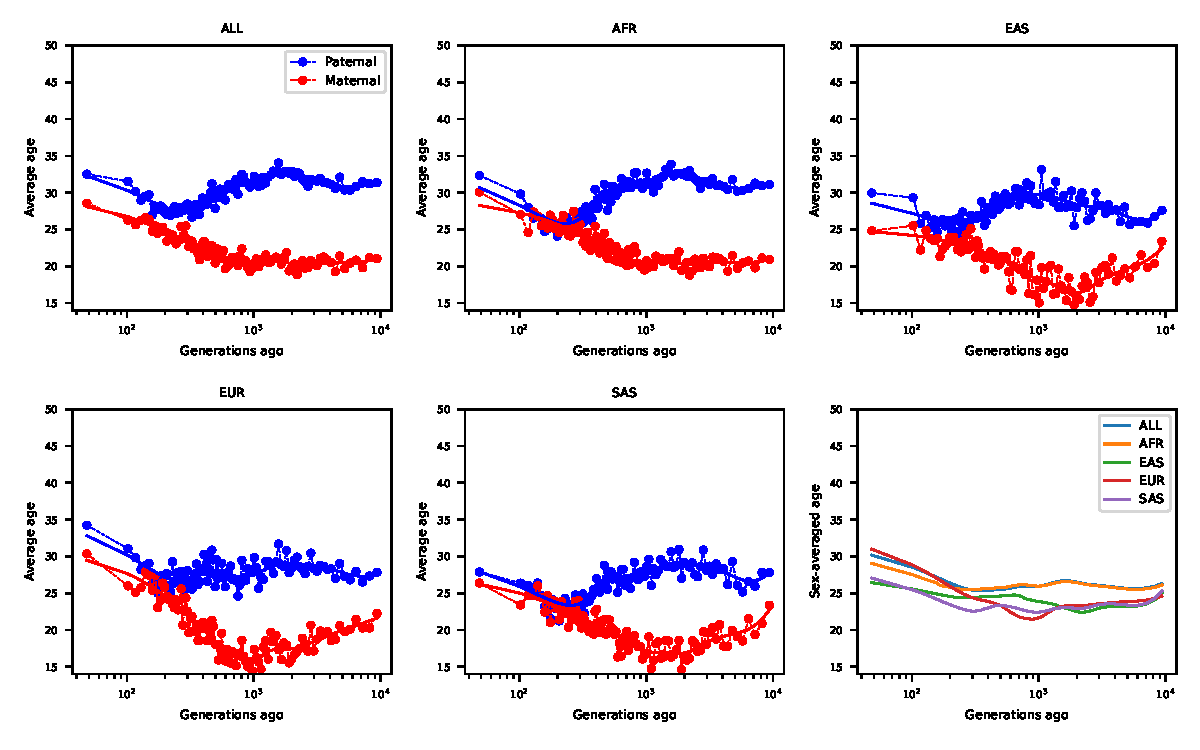
\includegraphics[width=0.8\textwidth]{../plots/inferred_generation_times.geva.max_age.10000.pdf}
    \caption{
        \textbf{\GEVA-inferred generation time histories.}
    }
    \label{fig:geva-gen-times}
\end{figure}


\begin{figure}[ht!]
    \centering
    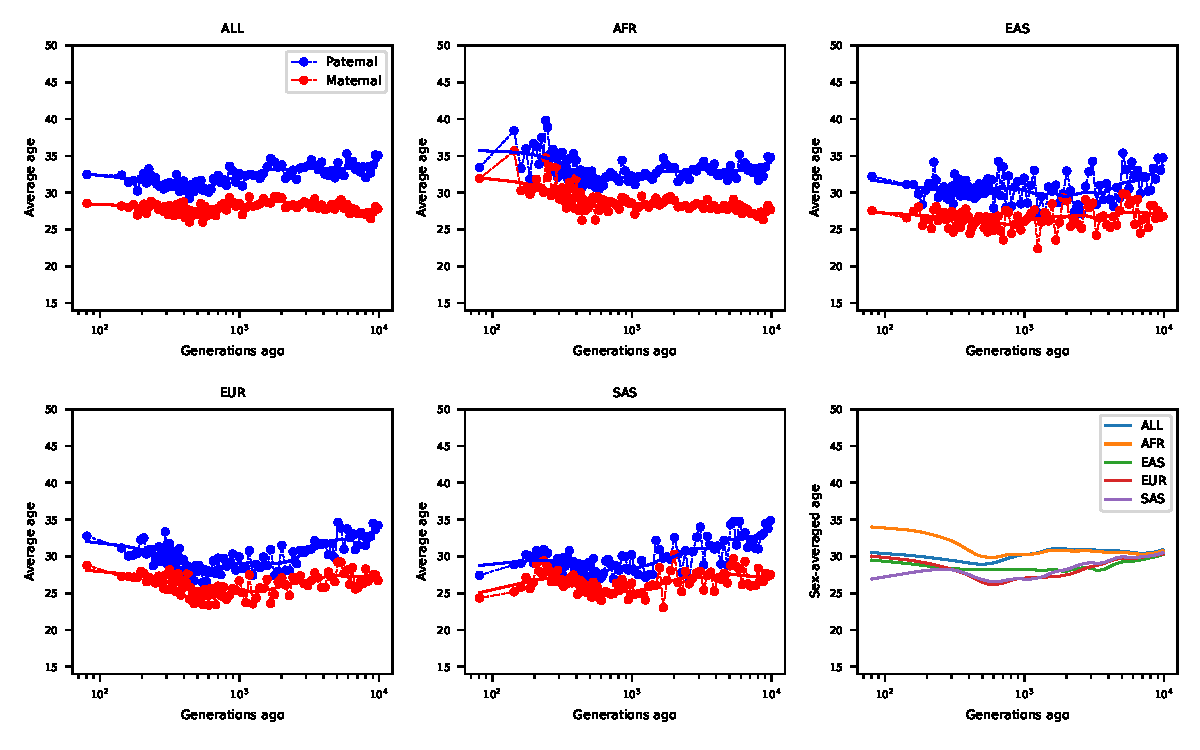
\includegraphics[width=0.8\textwidth]{../plots/inferred_generation_times.relate.pdf}
    \caption{
        \textbf{\relate-inferred generation time histories.}
    }
    \label{fig:relate-gen-times}
\end{figure}


\begin{figure}[ht!]
    \centering
    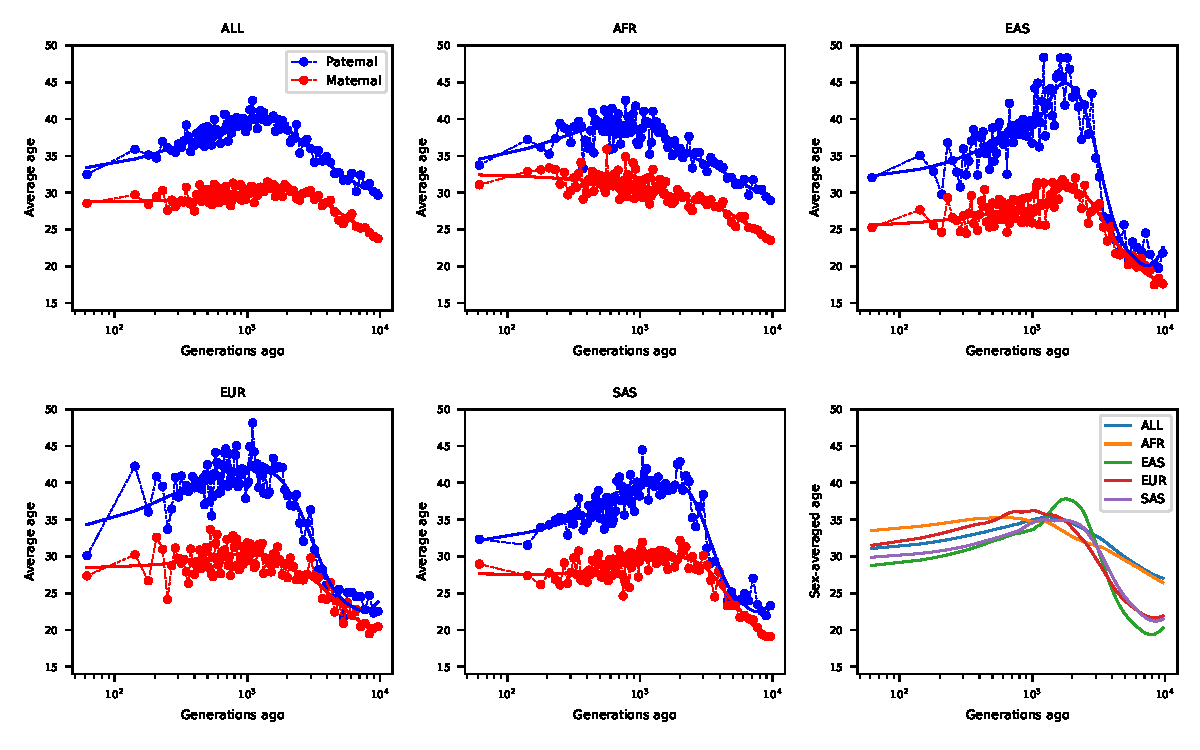
\includegraphics[width=0.8\textwidth]{../plots/inferred_generation_times.tsdate.pdf}
    \caption{
        \textbf{\tsdate-inferred generation time histories.}
    }
    \label{fig:tsdate-gen-times}
\end{figure}


\begin{figure}[ht!]
    \centering
    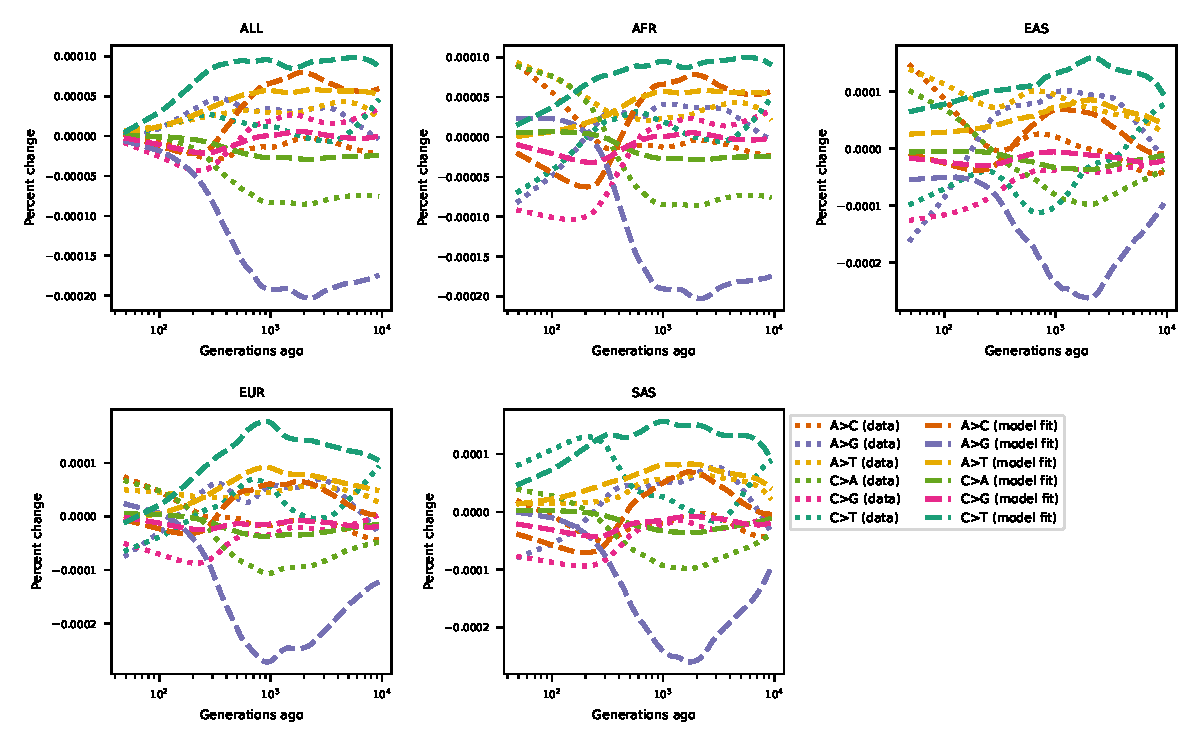
\includegraphics[width=0.8\textwidth]{../plots/goodness-of-fit.geva.max_age.10000.pdf}
    \caption{
        \textbf{Prediction of mutation spectrum history from
        \GEVA-inferred generation times.}
    }
    \label{fig:geva-fit}
\end{figure}


\begin{figure}[ht!]
    \centering
    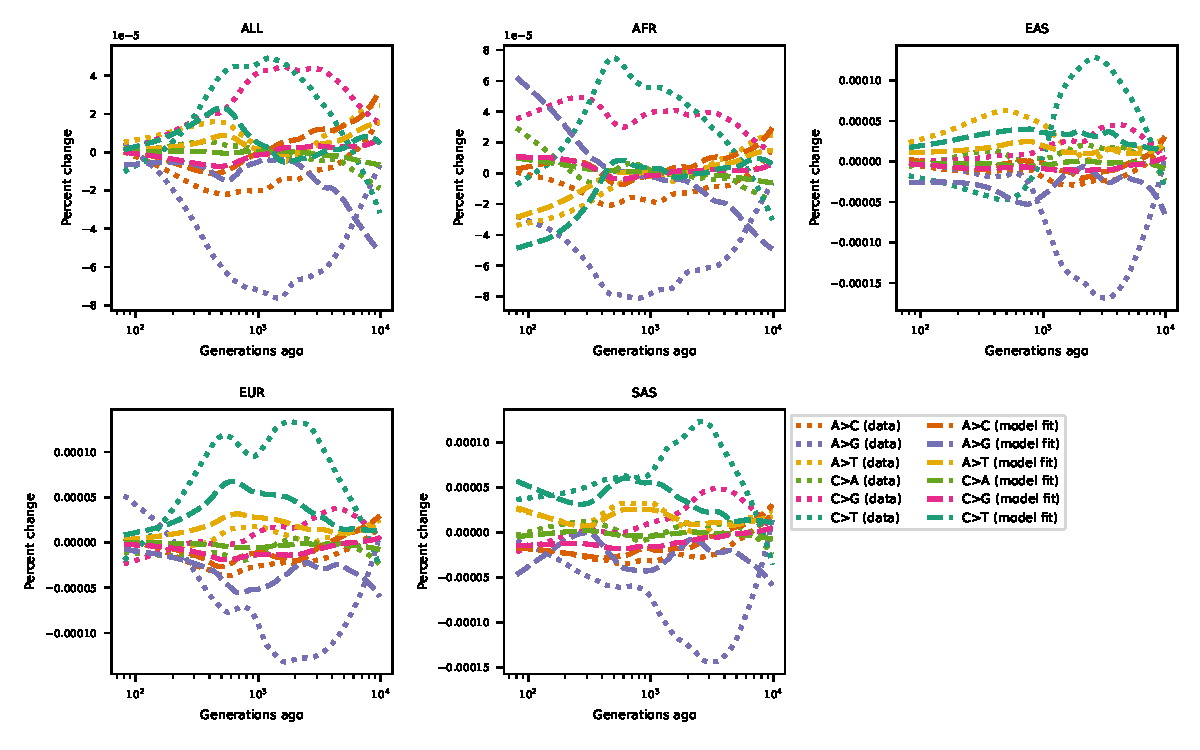
\includegraphics[width=0.8\textwidth]{../plots/goodness-of-fit.relate.pdf}
    \caption{
        \textbf{Prediction of mutation spectrum history from
        \relate-inferred generation times.}
    }
    \label{fig:relate-fit}
\end{figure}


\begin{figure}[ht!]
    \centering
    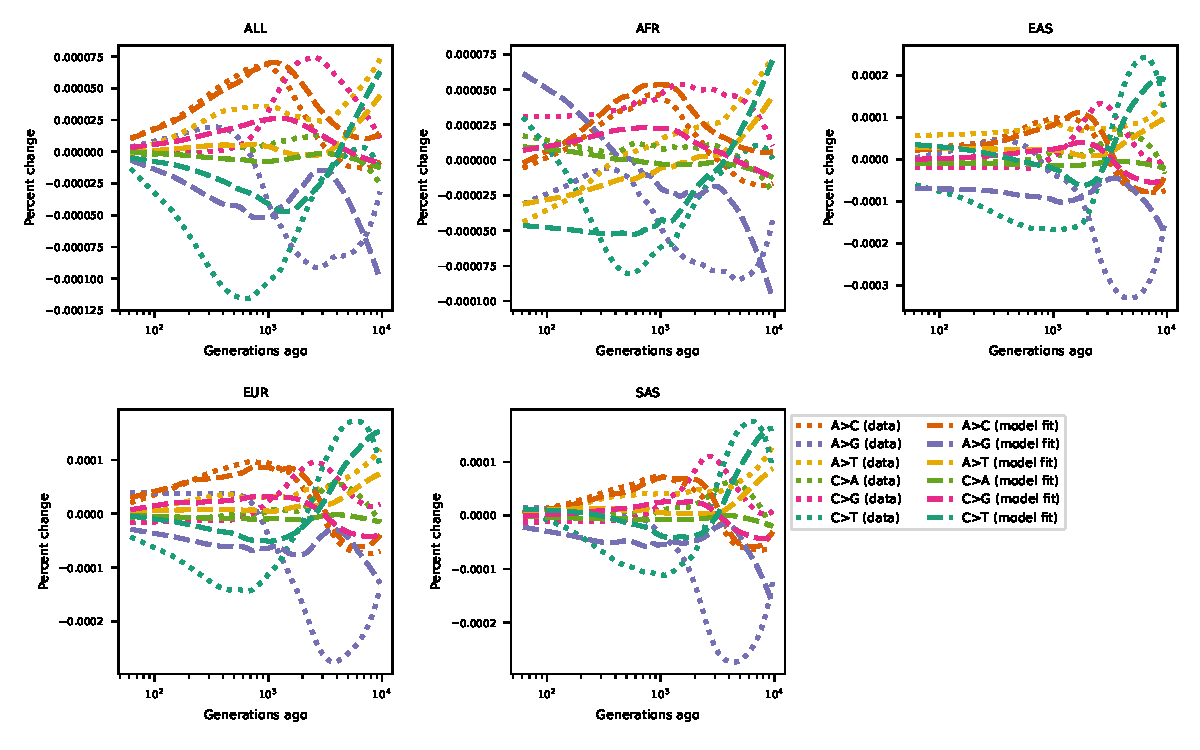
\includegraphics[width=0.8\textwidth]{../plots/goodness-of-fit.tsdate.pdf}
    \caption{
        \textbf{Prediction of mutation spectrum history from
        \tsdate-inferred generation times.}
    }
    \label{fig:tsdate-fit}
\end{figure}


\clearpage

\subsection*{Tables}

\begin{table}[h]
    \caption{
        \label{tab:recent-spectra}
        \textbf{Mutation profiles from the past 100 generations,
        compared to Iceland trios.}
        The most recent time bin for each method included the past $\approx150$
        generations. When singletons were included (when using data from
        \tsdate and \relate), the spectra of estimated
        recent standing variation were largely similar. Note that \GEVA
        does not report ages for singletons.
        While the three methods provide similar spectra from recent mutations,
        the spectrum from the Iceland trios differs substantially.
        The similarity in the spectrum between mutations that were phased
        in \citet{jonsson2017parental} and all mutations (phased and unphased)
        are very similar to each other.
    }
    \centering
    \begin{tabular}[t]{l|cccccc}
        \toprule
        Dataset & A$\rightarrow$C & A$\rightarrow$G & A$\rightarrow$T &
            C$\rightarrow$A & C$\rightarrow$G & C$\rightarrow$T \\
        \midrule
        \GEVA & 0.0946 & 0.3600 & 0.0886 & 0.1201 & 0.1057 & 0.2310 \\
        \tsdate & 0.0931 & 0.3579 & 0.0899 & 0.1146 & 0.1061 & 0.2384 \\
        \tsdate (w/singletons) & 0.0989 & 0.3598 & 0.0908 & 0.1168 & 0.1062 & 0.2275 \\
        \relate & 0.0991 & 0.3610 & 0.0863 & 0.1124 & 0.1038 & 0.2374 \\
        \relate (w/singletons) & 0.1002 & 0.3590 & 0.0921 & 0.1164 & 0.1060 & 0.2263 \\
        \midrule
        Trios (phased) & 0.1071 & 0.4100 & 0.0881 & 0.0481 & 0.0847 & 0.2620 \\
        Trios (all mutations) & 0.1080 & 0.4086 & 0.0903 & 0.0483 & 0.0839 & 0.2610 \\
        \bottomrule
    \end{tabular}
\end{table}

\clearpage

\bibliographystyle{genetics}
\bibliography{doc}

\end{document}
